\documentclass[border=3pt]{standalone}
% Shared preamble for standalone figures (same fonts/colours as the paper).
\usepackage[T1]{fontenc}
\usepackage{lmodern}
\usepackage{amsmath,amssymb}
\usepackage[dvipsnames,svgnames]{xcolor}
\usepackage{tikz}
\usetikzlibrary{arrows.meta,positioning,calc,shapes.geometric,decorations.pathreplacing,shadings}
\usepackage{pgfplots}
\pgfplotsset{compat=1.18}
\usepgfplotslibrary{fillbetween}
\definecolor{pgrey}{HTML}{EEEEEE}
\definecolor{ppink}{HTML}{F8D7DA}
\definecolor{ppeach}{HTML}{FDE5C8}
\definecolor{porange}{HTML}{FBC78D}
\definecolor{pgreen}{HTML}{D4F7D4}
\definecolor{ppurple}{HTML}{EFE3F7}
\definecolor{pblue}{HTML}{DCE8F7}
\definecolor{dgreen}{HTML}{2E8B2E}
\definecolor{dpink}{HTML}{C2185B}
\definecolor{dorange}{HTML}{E07B00}
\definecolor{dblue}{HTML}{1F4E9E}
\definecolor{dpurple}{HTML}{7B3FA0}
\definecolor{gold}{HTML}{E0A800}
\tikzset{
  blk/.style={draw=black!70,rounded corners=2pt,minimum height=0.8cm,minimum width=1.9cm,
              align=center,font=\sffamily\footnotesize,inner sep=3pt},
  arr/.style={-{Stealth[length=2.2mm]},thick,black!75},
  darr/.style={-{Stealth[length=2mm]},dashed,thick},
  lbl/.style={font=\itshape\scriptsize},
}

\begin{document}
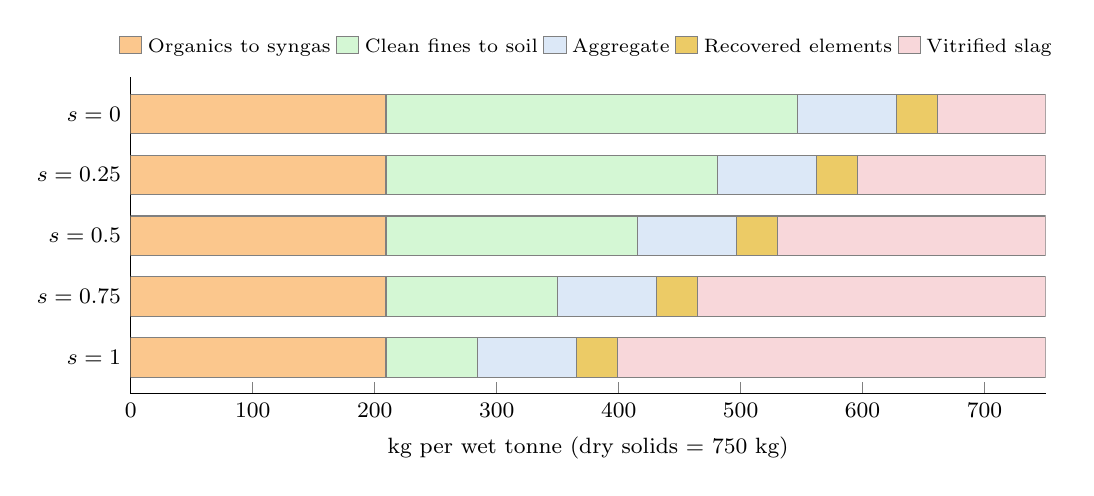
\begin{tikzpicture}
\begin{axis}[xbar stacked, width=13.2cm, height=5.6cm, bar width=0.5cm,
  xmin=0, xmax=750, ytick=data,
  yticklabels={{$s=0$},{$s=0.25$},{$s=0.5$},{$s=0.75$},{$s=1$}},
  y dir=reverse, xlabel={kg per wet tonne (dry solids = 750 kg)},
  legend style={at={(0.5,1.03)},anchor=south,legend columns=5,font=\scriptsize,draw=none},
  tick label style={font=\footnotesize}, label style={font=\footnotesize},
  enlarge y limits=0.15, axis x line*=bottom, axis y line*=left]
\addplot[fill=porange,draw=black!50] coordinates {(209.25,0) (209.25,1) (209.25,2) (209.25,3) (209.25,4)};
\addlegendentry{Organics to syngas}
\addplot[fill=pgreen,draw=black!50] coordinates {(337.5,0) (271.875,1) (206.25,2) (140.625,3) (75,4)};
\addlegendentry{Clean fines to soil}
\addplot[fill=pblue,draw=black!50] coordinates {(81,0) (81,1) (81,2) (81,3) (81,4)};
\addlegendentry{Aggregate}
\addplot[fill=gold!60,draw=black!50] coordinates {(33.696,0) (33.743,1) (33.743,2) (33.900,3) (33.900,4)};
\addlegendentry{Recovered elements}
\addplot[fill=ppink,draw=black!50] coordinates {(88.554,0) (154.132,1) (219.757,2) (285.225,3) (350.850,4)};
\addlegendentry{Vitrified slag}
\legend{Organics to syngas, Clean fines to soil, Aggregate, Recovered elements, Vitrified slag}
\end{axis}
\end{tikzpicture}
\end{document}
